\documentclass[12pt,a4paper]{book}

\usepackage[francais]{babel}
\usepackage[utf8]{inputenc}
\usepackage{epigraph}
\usepackage[T1]{fontenc}
\usepackage{listings}
\usepackage{graphicx}
\usepackage{parskip}
\graphicspath{{images/}}

%%macro

\newcommand{\path}[1]{\texttt{#1}}

\begin{document}
\title{{\huge Inititation à la programmation}}
\author{Bastien Gorissen \& Thomas Stassin}
\date{Année 2016}

\maketitle

\chapter{Level 1}

%%<Mettre ici tout la partie introduction>

\section{Qu’est-ce qu’un langage de programmation?}

\epigraph{Un langage de programmation est une convention pour donner des ordres à un ordinateur. Ce n’est pas censé être obscur, bizarre et plein de pièges subtils.
Ca, ce sont les caractéristiques de la magie.}{\textit{Dave Small}}

Un langage de programmation est un moyen d’intéragir avec l’ordinateur afin de lui donner des instructions, le langage qui est \emph{intelligible}, 
sera \emph{interprété} afin d’être compris par la machine.

\begin{figure}[ht]
\centering
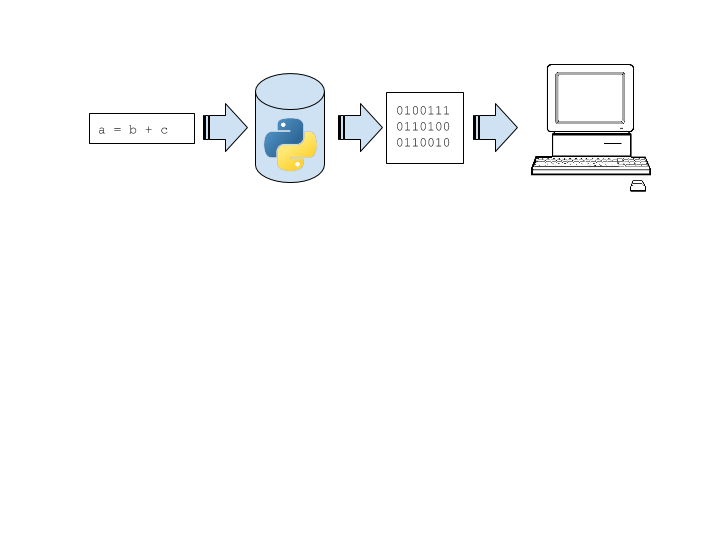
\includegraphics[scale=0.5]{translate_code.png} 
\end{figure}

\subsection{Exercice}
 
Executer le script se trouvant dans le dossier \path{<dossier\_path>}

\section{Commander à l'ordinateur}

Pour ``commander'' l’ordinateur, on lui donne des \emph{instructions}, le plus souvent, c’est instructions seront regroupées dans un \emph{script}.

\subsection{Exercice}

Dans l’exercice précédent, nous avons exécuté le script \path{<script\_name>}, ce script est remplie d’instructions, dont celle-ci:

%%ajouter code qui définit les dimensions du donjons

Que ce passerait t’il si on modifiait l’instruction dans le script?

\end{document}

Matière:
Les variables (première approche)
conversion d’une variable en chaine de caractère (str)

Exercice:
Utiliser l'instruction de sortie pour afficher les dimension du monde dans la console
Utiliser la variable du héro pour le bouger par script

Bonus Stage:
    Faire sortir le héros par script du stage.

Level 1

<Mettre ici tout la partie introduction>

Qu’est-ce qu’un langage de programmation?

Un langage de programmation est une convention pour donner des ordres à un ordinateur. Ce n’est pas censé être obscur, bizarre et plein de pièges subtils. Ca, ce sont les caractéristiques de la magie.

    - Dave Small


Un langage de programmation est un moyen d’intéragir avec l’ordinateur afin de lui donner des instructions, le langage qui est  “intelligible”, sera “interprété” afin d’être compris par la machine.





Pour “commander” l’ordinateur, on lui donne des instructions, le plus souvent, c’est    instructions seront regroupées dans un script.
Dans l’exercice précédent, nous avons exécuté le script <script_name>, ce script est remplie d’instructions, dont celle-ci:

<Ajouter ici le code qui definit la dimension du donjon>


Que ce passerait t’il si on modifiait l’instruction dans le script.

Exercice 2:
Changez les données de dimension du donjon dans le script.


Il existe plusieurs sorte d’instruction, l’une d’elles sont les instructions de sortie.
Une instruction de sortie envoie vers une “sortie” se qu’on lui donne.
Une des sortie les plus couramment utilisé est la console et Python, l’instruction de sortie vers la console est print

Et donc voici le classique, mais indémodable “Hello World” en Python

print(‘Hello World!’)

Exercice 3:

Lorsque le donjon est créé, signalez-le par un message dans la console.


Souvent, il sera utile de stocké certaines valeur tout au long de l’éxécution de votre code.
Par exemple pour stocké la valeur d’un calcul, où même afin de réutilisé ses valeurs plusieurs fois. Pour stocker les valeurs, on utilise des variables.

La variables est un moyen de stocké une valeur quelconque (un nombre, du texte, voir même des objets plus complexes) dans la mémoire du programme.

Dans le cas de notre jeu, le donjon, ainsi que le héro sont contenu chacun dans une variable.

<Montrer les lignes de code>

En Python, l’affectation d’une valeur se fait avec l’opérateur =

Dans a=3, On affecte 3 à la variable a



Exercices 4:
